\documentclass[a4paper]{article}
\usepackage[]{graphicx}\usepackage[]{color}
% maxwidth is the original width if it is less than linewidth
% otherwise use linewidth (to make sure the graphics do not exceed the margin)
\makeatletter
\def\maxwidth{ %
  \ifdim\Gin@nat@width>\linewidth
    \linewidth
  \else
    \Gin@nat@width
  \fi
}
\makeatother

\definecolor{fgcolor}{rgb}{0.345, 0.345, 0.345}
\newcommand{\hlnum}[1]{\textcolor[rgb]{0.686,0.059,0.569}{#1}}%
\newcommand{\hlstr}[1]{\textcolor[rgb]{0.192,0.494,0.8}{#1}}%
\newcommand{\hlcom}[1]{\textcolor[rgb]{0.678,0.584,0.686}{\textit{#1}}}%
\newcommand{\hlopt}[1]{\textcolor[rgb]{0,0,0}{#1}}%
\newcommand{\hlstd}[1]{\textcolor[rgb]{0.345,0.345,0.345}{#1}}%
\newcommand{\hlkwa}[1]{\textcolor[rgb]{0.161,0.373,0.58}{\textbf{#1}}}%
\newcommand{\hlkwb}[1]{\textcolor[rgb]{0.69,0.353,0.396}{#1}}%
\newcommand{\hlkwc}[1]{\textcolor[rgb]{0.333,0.667,0.333}{#1}}%
\newcommand{\hlkwd}[1]{\textcolor[rgb]{0.737,0.353,0.396}{\textbf{#1}}}%
\let\hlipl\hlkwb

\usepackage{framed}
\makeatletter
\newenvironment{kframe}{%
 \def\at@end@of@kframe{}%
 \ifinner\ifhmode%
  \def\at@end@of@kframe{\end{minipage}}%
  \begin{minipage}{\columnwidth}%
 \fi\fi%
 \def\FrameCommand##1{\hskip\@totalleftmargin \hskip-\fboxsep
 \colorbox{shadecolor}{##1}\hskip-\fboxsep
     % There is no \\@totalrightmargin, so:
     \hskip-\linewidth \hskip-\@totalleftmargin \hskip\columnwidth}%
 \MakeFramed {\advance\hsize-\width
   \@totalleftmargin\z@ \linewidth\hsize
   \@setminipage}}%
 {\par\unskip\endMakeFramed%
 \at@end@of@kframe}
\makeatother

\definecolor{shadecolor}{rgb}{.97, .97, .97}
\definecolor{messagecolor}{rgb}{0, 0, 0}
\definecolor{warningcolor}{rgb}{1, 0, 1}
\definecolor{errorcolor}{rgb}{1, 0, 0}
\newenvironment{knitrout}{}{} % an empty environment to be redefined in TeX

\usepackage{alltt}
\newcommand{\SweaveOpts}[1]{}  % do not interfere with LaTeX
\newcommand{\SweaveInput}[1]{} % because they are not real TeX commands
\newcommand{\Sexpr}[1]{}       % will only be parsed by R



\usepackage[utf8]{inputenc}
\pagenumbering{arabic}
%\usepackage[ngerman]{babel}
\usepackage{a4wide,paralist}
\usepackage{amsmath, amssymb, xfrac, amsthm}
\usepackage{dsfont}
\usepackage[usenames,dvipsnames]{xcolor}
\usepackage{amsfonts}
\usepackage{graphicx}
\usepackage{caption}
\usepackage{subcaption}
\usepackage{framed}
\usepackage{multirow}
\usepackage{bytefield}
\usepackage{csquotes}
\usepackage[breakable, theorems, skins]{tcolorbox}
\usepackage{hyperref}
\usepackage{cancel}
\usepackage{bm}

\input{../../style/common}

\tcbset{enhanced}

%exercise numbering
\renewcommand{\theenumi}{(\alph{enumi})}
\renewcommand{\theenumii}{\roman{enumii}}
\renewcommand\labelenumi{\theenumi}

\font \sfbold=cmssbx10
\setlength{\oddsidemargin}{0cm} \setlength{\textwidth}{16cm}

\sloppy
\parindent0em
\parskip0.5em
\topmargin-2.3 cm
\textheight25cm
\textwidth17.5cm
\oddsidemargin-0.8cm
% \pagestyle{empty}

\newcommand{\kopf}[1] {
\hrule
\vspace{.15cm}
\begin{minipage}{\textwidth}
	{\sf \bf \huge Exercise Collection -- #1}
\end{minipage}
\vspace{.05cm}
\hrule
\vspace{1cm}}

\newcommand{\exlect}
  {\color{black} \hrule \section{Lecture exercises}}
  
\newcommand{\exexams}
  {\color{black} \hrule \section{Questions from past exams}}
  
\newcommand{\exinspo}
  {\color{black} \hrule \section{Ideas \& exercises from other sources}}

\newcounter{aufg}
\newenvironment{aufgabe}[1]
	{\color{black} \refstepcounter{aufg}
	\subsection{Exercise \arabic{aufg}: #1} 
	\noindent}
	{\vspace{0.5cm}}
	
\newenvironment{aufgabeexam}[3] % semester, main or retry exam, question number
	{\color{black} \refstepcounter{aufg}
	\subsection{Exercise \arabic{aufg}: #1, #2 exam, question #3}
	\noindent}
	{\vspace{1.5cm}}

\newcounter{loes}
\newenvironment{loesung}
	{\color{gray} \refstepcounter{loes}\textbf{Solution \arabic{loes}:}
	\\ \noindent}
	{\bigskip}

\setcounter{secnumdepth}{0}



\begin{document}
% !Rnw weave = knitr



\input{../../latex-math/basic-math.tex}
\input{../../latex-math/basic-ml.tex}

\kopf{Supervised Regression}

\tableofcontents

% ------------------------------------------------------------------------------
% LECTURE EXERCISES
% ------------------------------------------------------------------------------

\dlz
\exlect
\lz

\aufgabe{$k$-NN regression}{

%x <- c(4,7,9,4,6,7,9,7,8)
%y <- c(6,3,8,9,5,8,7,6,5)
%z <- as.factor(c(1,1,1,0,0,0,0,2,1))

Let the 2D feature vectors in the following figure be with two different numeric target values (2 and 4). Predict the point (7,6) - represented by the grey point in the picture - with the k-nearest neighbor method. Distance function should be the $L_1$ norm (Manhattan distance):

$$d_\text{manhattan}(x, \tilde{x}) = \sum_{j=1}^p |x_j - \tilde{x}_j|$$

State as the prediction the unweighted and the weighted (according to the Manhattan distance) mean of the values of the k-nearest neighbors.

\begin{itemize}
  \item[a)] $k = 3$
  \item[b)] $k = 5$
  \item[c)] $k = 7$
\end{itemize}

%d3 = c(5,7,9,7)
%v3 = c(6,8,6,4)

%d5 = c(4,7,10,7)
%v5 = c(6,9,6,3)

%d7 = c(3,7,10,10,7)
%v7 = c(6,10,7,5,2)



\begin{knitrout}
\definecolor{shadecolor}{rgb}{0.969, 0.969, 0.969}\color{fgcolor}

{\centering 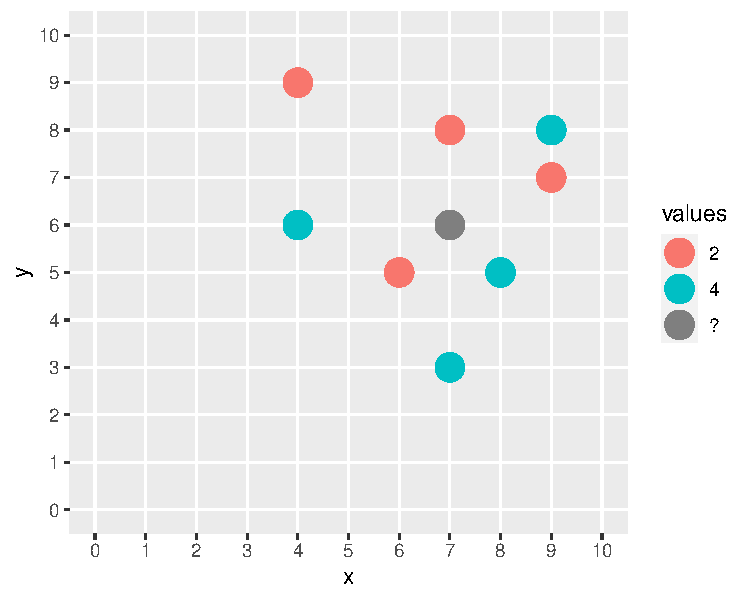
\includegraphics[width=\maxwidth]{figure/unnamed-chunk-8-1} 

}


\end{knitrout}
}

\dlz
\loesung{

\begin{enumerate}
\item[a)] $k = 3$
\begin{align*}
\hat{y} =& \frac{2 + 2 + 4}{3} = \frac{8}{3} \approx 2.67\\
\hat{y}_\mathrm{weighted} =& \frac{\frac{1}{2}\cdot 2 + \frac{1}{2}\cdot 2 + \frac{1}{2}\cdot 4}{\frac{3}{2}} = \frac{8}{3} \approx 2.67 \\
\end{align*}

\begin{knitrout}
\definecolor{shadecolor}{rgb}{0.969, 0.969, 0.969}\color{fgcolor}

{\centering 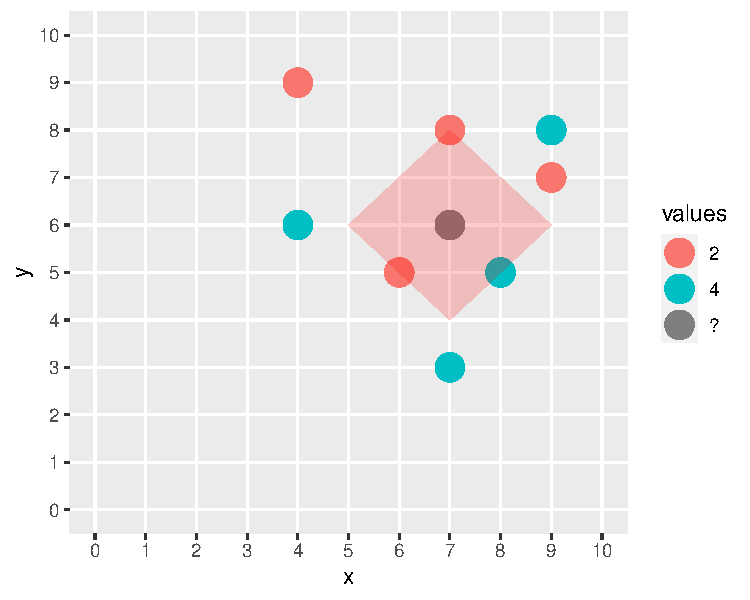
\includegraphics[width=\maxwidth]{figure/unnamed-chunk-9-1} 

}


\end{knitrout}

\item[b)] $k = 5$

\begin{align*}
\hat{y} =& \frac{2 + 2 + 2 + 4 + 4 + 4}{6} = 3 \\
\hat{y}_\mathrm{weighted} =& \frac{\frac{1}{2}\cdot 2 + \frac{1}{2}\cdot2 + \frac{1}{3} \cdot 2 +  \frac{1}{2}\cdot 4 + \frac{1}{3}\cdot 4 + \frac{1}{3}\cdot 4}{\frac{5}{2}} = \frac{44}{15} \approx 2.93\\
\end{align*}

\begin{knitrout}
\definecolor{shadecolor}{rgb}{0.969, 0.969, 0.969}\color{fgcolor}

{\centering 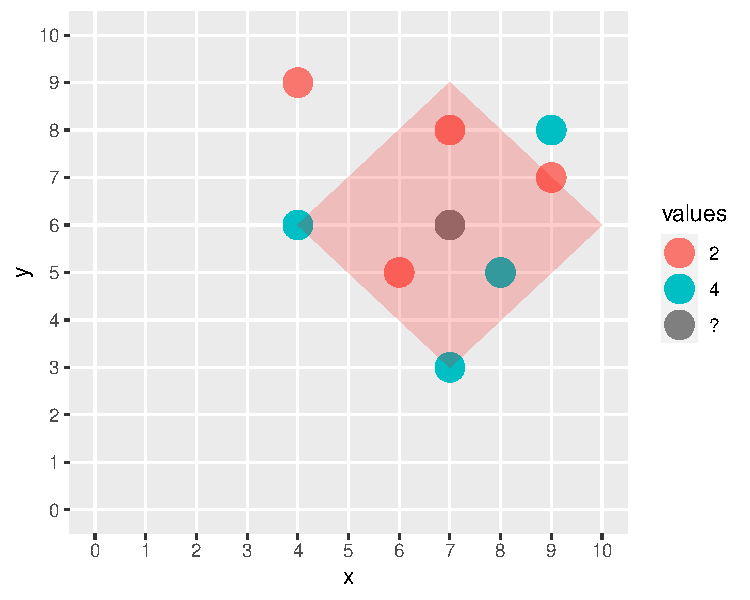
\includegraphics[width=\maxwidth]{figure/unnamed-chunk-10-1} 

}


\end{knitrout}

\item[c)] $k = 7$

\begin{align*}
\hat{y} =& \frac{2 + 2 + 2 + 4 + 4 + 4 + 4}{7} = \frac{22}{7} \approx 3.14\\
\hat{y}_\mathrm{weighted} =& \frac{\frac{1}{2}\cdot 2 + \frac{1}{2}\cdot2 + \frac{1}{3} \cdot 2 +  \frac{1}{2}\cdot 4 + \frac{1}{3}\cdot 4 + \frac{1}{3}\cdot 4 + \frac{1}{4} \cdot 4}{\frac{11}{4}} = \frac{100}{33} \approx 3.03\\
\end{align*}

\begin{knitrout}
\definecolor{shadecolor}{rgb}{0.969, 0.969, 0.969}\color{fgcolor}

{\centering 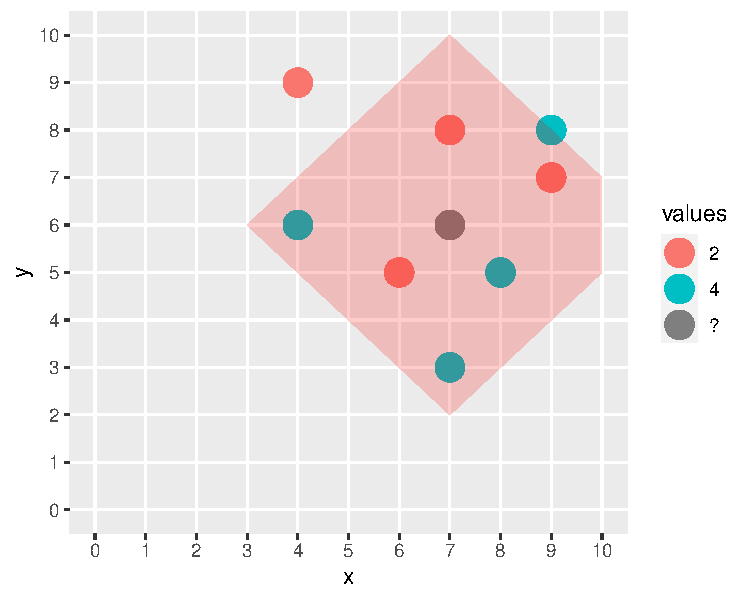
\includegraphics[width=\maxwidth]{figure/unnamed-chunk-11-1} 

}


\end{knitrout}

\end{enumerate}


  
}

\newpage

\aufgabe{\texttt{mlr3} regression learners}{

How in mlr3 a learner can be constructed and what it represents can be found 
at \url{https://mlr3book.mlr-org.com/learners.html}.
\begin{enumerate}
\item[a)] How does a learner in mlr3 compare to what you've learned in the videos?
\item[b)] Pick an mlr3 learner of your choice. What are the different settings for this learner? \\ 
(Hint: Use \texttt{mlr\_learners\$keys()} to see all available learners)
\end{enumerate}
}
\dlz
\loesung{

\begin{enumerate}
\item[a)] Learning consists of \textit{representation} (hypothesis space), 
\textit{evaluation} (risk) and \textit{optimization}. \\
A learner in mlr3 can be thought of as the implementation of these components, 
since 
\begin{itemize}
\item a representation of the associated model learnt from the data by 
using the implemented optimization is stored in such a learner object,
\item its performance measures can be accessed afterwards.
\end{itemize}
\item[b)] 
\begin{knitrout}
\definecolor{shadecolor}{rgb}{0.969, 0.969, 0.969}\color{fgcolor}\begin{kframe}
\begin{alltt}
\hlkwd{library}\hlstd{(mlr3)}
\hlkwd{library}\hlstd{(mlr3learners)}

\hlcom{# show all available learners}
\hlstd{mlr_learners}\hlopt{$}\hlkwd{keys}\hlstd{()}
\end{alltt}
\begin{verbatim}
##  [1] "classif.cv_glmnet"   "classif.debug"       "classif.featureless"
##  [4] "classif.glmnet"      "classif.kknn"        "classif.lda"        
##  [7] "classif.log_reg"     "classif.multinom"    "classif.naive_bayes"
## [10] "classif.nnet"        "classif.qda"         "classif.ranger"     
## [13] "classif.rpart"       "classif.svm"         "classif.xgboost"    
## [16] "regr.cv_glmnet"      "regr.featureless"    "regr.glmnet"        
## [19] "regr.kknn"           "regr.km"             "regr.lm"            
## [22] "regr.ranger"         "regr.rpart"          "regr.svm"           
## [25] "regr.xgboost"        "surv.cv_glmnet"      "surv.glmnet"        
## [28] "surv.ranger"         "surv.xgboost"
\end{verbatim}
\begin{alltt}
\hlcom{# see settings for a specific learner, e.g., for a regression tree}
\hlstd{rpart_learner} \hlkwb{<-} \hlkwd{lrn}\hlstd{(}\hlstr{"regr.rpart"}\hlstd{)}
\hlkwd{print}\hlstd{(rpart_learner)}
\end{alltt}
\begin{verbatim}
## <LearnerRegrRpart:regr.rpart>
## * Model: -
## * Parameters: xval=0
## * Packages: rpart
## * Predict Type: response
## * Feature types: logical, integer, numeric, factor, ordered
## * Properties: importance, missings, selected_features, weights
\end{verbatim}
\end{kframe}
\end{knitrout}


\end{enumerate}
}

\newpage

\aufgabe{regression for \texttt{abalone} data}{

We want to predict the age of an abalone using its longest shell measurement and its weight.

See: \url{http://archive.ics.uci.edu/ml/datasets/Abalone} for more details.

\begin{itemize}
  \item[a)] Plot \texttt{LongestShell}, \texttt{WholeWeight} on the $x$- and $y$-axis and color points with \texttt{Rings}
\end{itemize}

  Using the mlr3-package:

\begin{itemize}
  \item[b)] Fit a linear model
  \item[c)] Fit a k-nearest-neighbors model
  \item[d)] Compare the fitted and observed targets for lm and knn, respectively (Hint: Use \texttt{autoplot()})
  % \item[e)] Compare which model performs better.
\end{itemize}

Hint: See the official book manual of the mlr3 package for usage:
\begin{center}
\url{https://mlr3book.mlr-org.com/index.html}
\end{center}
}
\dlz
\loesung{

See 
\href{https://github.com/compstat-lmu/lecture_i2ml/blob/master/exercises/supervised-regression/ex_rnw/sol_knn_lm.R}{R code}
}

% ------------------------------------------------------------------------------
% PAST EXAMS
% ------------------------------------------------------------------------------

\dlz
\exexams
\lz

\aufgabeexam{WS2020/21}{retry}{1}{

\begin{tabular}{ | c | c | c |}
\hline
ID  &  $\xv$  &  $y$  \\  \hline
1   &  0.0    &  0.0  \\
2   &  1.0    &  4.0  \\
3   &  1.5    &  5.5  \\
4   &  2.5    &  7.0  \\
5   &  3.5    &  6.0  \\
6   &  5.0    &  3.0  \\
7   &  6.0    &  2.0  \\
8   &  7.0    &  3.0  \\
9   &  8.0    &  8.0  \\
\hline
\end{tabular}

\begin{centering}



\end{centering}

\begin{knitrout}
\definecolor{shadecolor}{rgb}{0.969, 0.969, 0.969}\color{fgcolor}
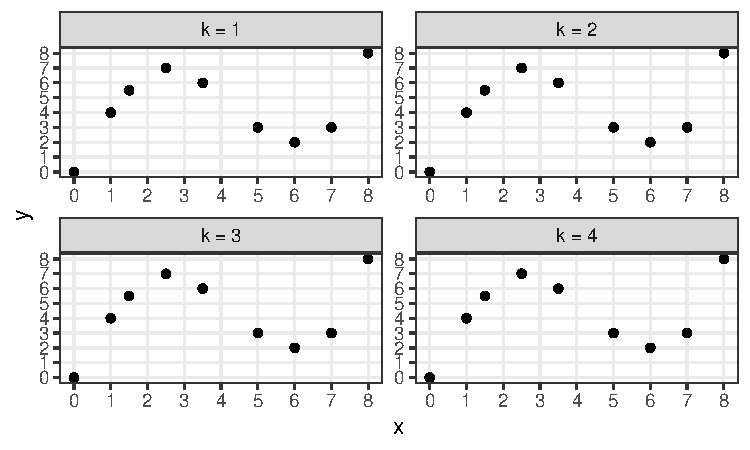
\includegraphics[width=\maxwidth]{figure/unnamed-chunk-7-1} 
\end{knitrout}

\begin{enumerate}
  \item Assume we use k-nearest neighbours regression with the L1 norm 
  (Manhattan distance) as a distance function. For every $k \in \{1, 2, 3, 4\}$, 
  do the following: 
  \begin{enumerate}
    \item[(i)] Mark the k-nearest neighbours of a new observation $\xv=4$ in the 
    graphic below. 
    \item[(ii)] Calculate the predicted value $\hat{y}$ for $\xv=4$ as the 
    unweighted mean of the k-nearest neighbours and draw it in the graphic 
    below.
  \end{enumerate}
  \item Would using the euclidean distance as distance measure in a) have made 
  a difference? Explain your answer.
\end{enumerate}  

\dlz

\loesung{

\begin{enumerate}
  \item $\{x_5\}$, $\{x_5, x_6\}$, $\{x_4, x_5, x_6\}$, $\{x_4, x_5, x_6, x_7\}$
  \item No. In the case of a single feature L1 and L2 are identical.
\end{enumerate} 
}

% ------------------------------------------------------------------------------
% INSPO
% ------------------------------------------------------------------------------

\dlz
\exinspo
\end{document}
